\begin{center}
    \addcontentsline{toc}{section}{Тэарэтычнае абгрунтаванне}
    \section*{Тэарэтычнае абгрунтаванне}    
\end{center}

У гэтай частцы курсавога праэкта будзе тэарэтычна апісаная задача рэканструкцыі паверхні, разгледжаныя этапы яе рашэння. Будзе апісаная як агульная задача, так і асаблівасці рашэння задачы пры наяўнасці дадатковых дадзеных.\par

\vspace{5mm}

Задачу рэканструкцыі паверхні (задачу рэканструкцыі любога трохмернага аб'екта) можна падзяліць на некалькі этапаў:
\begin{itemize}
    \item вылучэнне ключавых кропак (англ. Feature Extraction),
    \item спалучэнне кропак на розных выявах, якія адпавядаюць адной і той жа кропцы прасторы (англ. Feature Matching),
    \item пабудова разрэджанага воблака кропак на аснове спалучэнняў, атрыманых на папярэднім этапе рэканструкцыі,
    \item ушчыльненне атрыманага воблака, нанясенне тэкстураў і г.д.
\end{itemize}

\addcontentsline{toc}{subsection}{Вылучэнне ключавых кропак}
\subsection*{Вылучэнне ключавых кропак}

\begin{figure}[h]
    \centering
    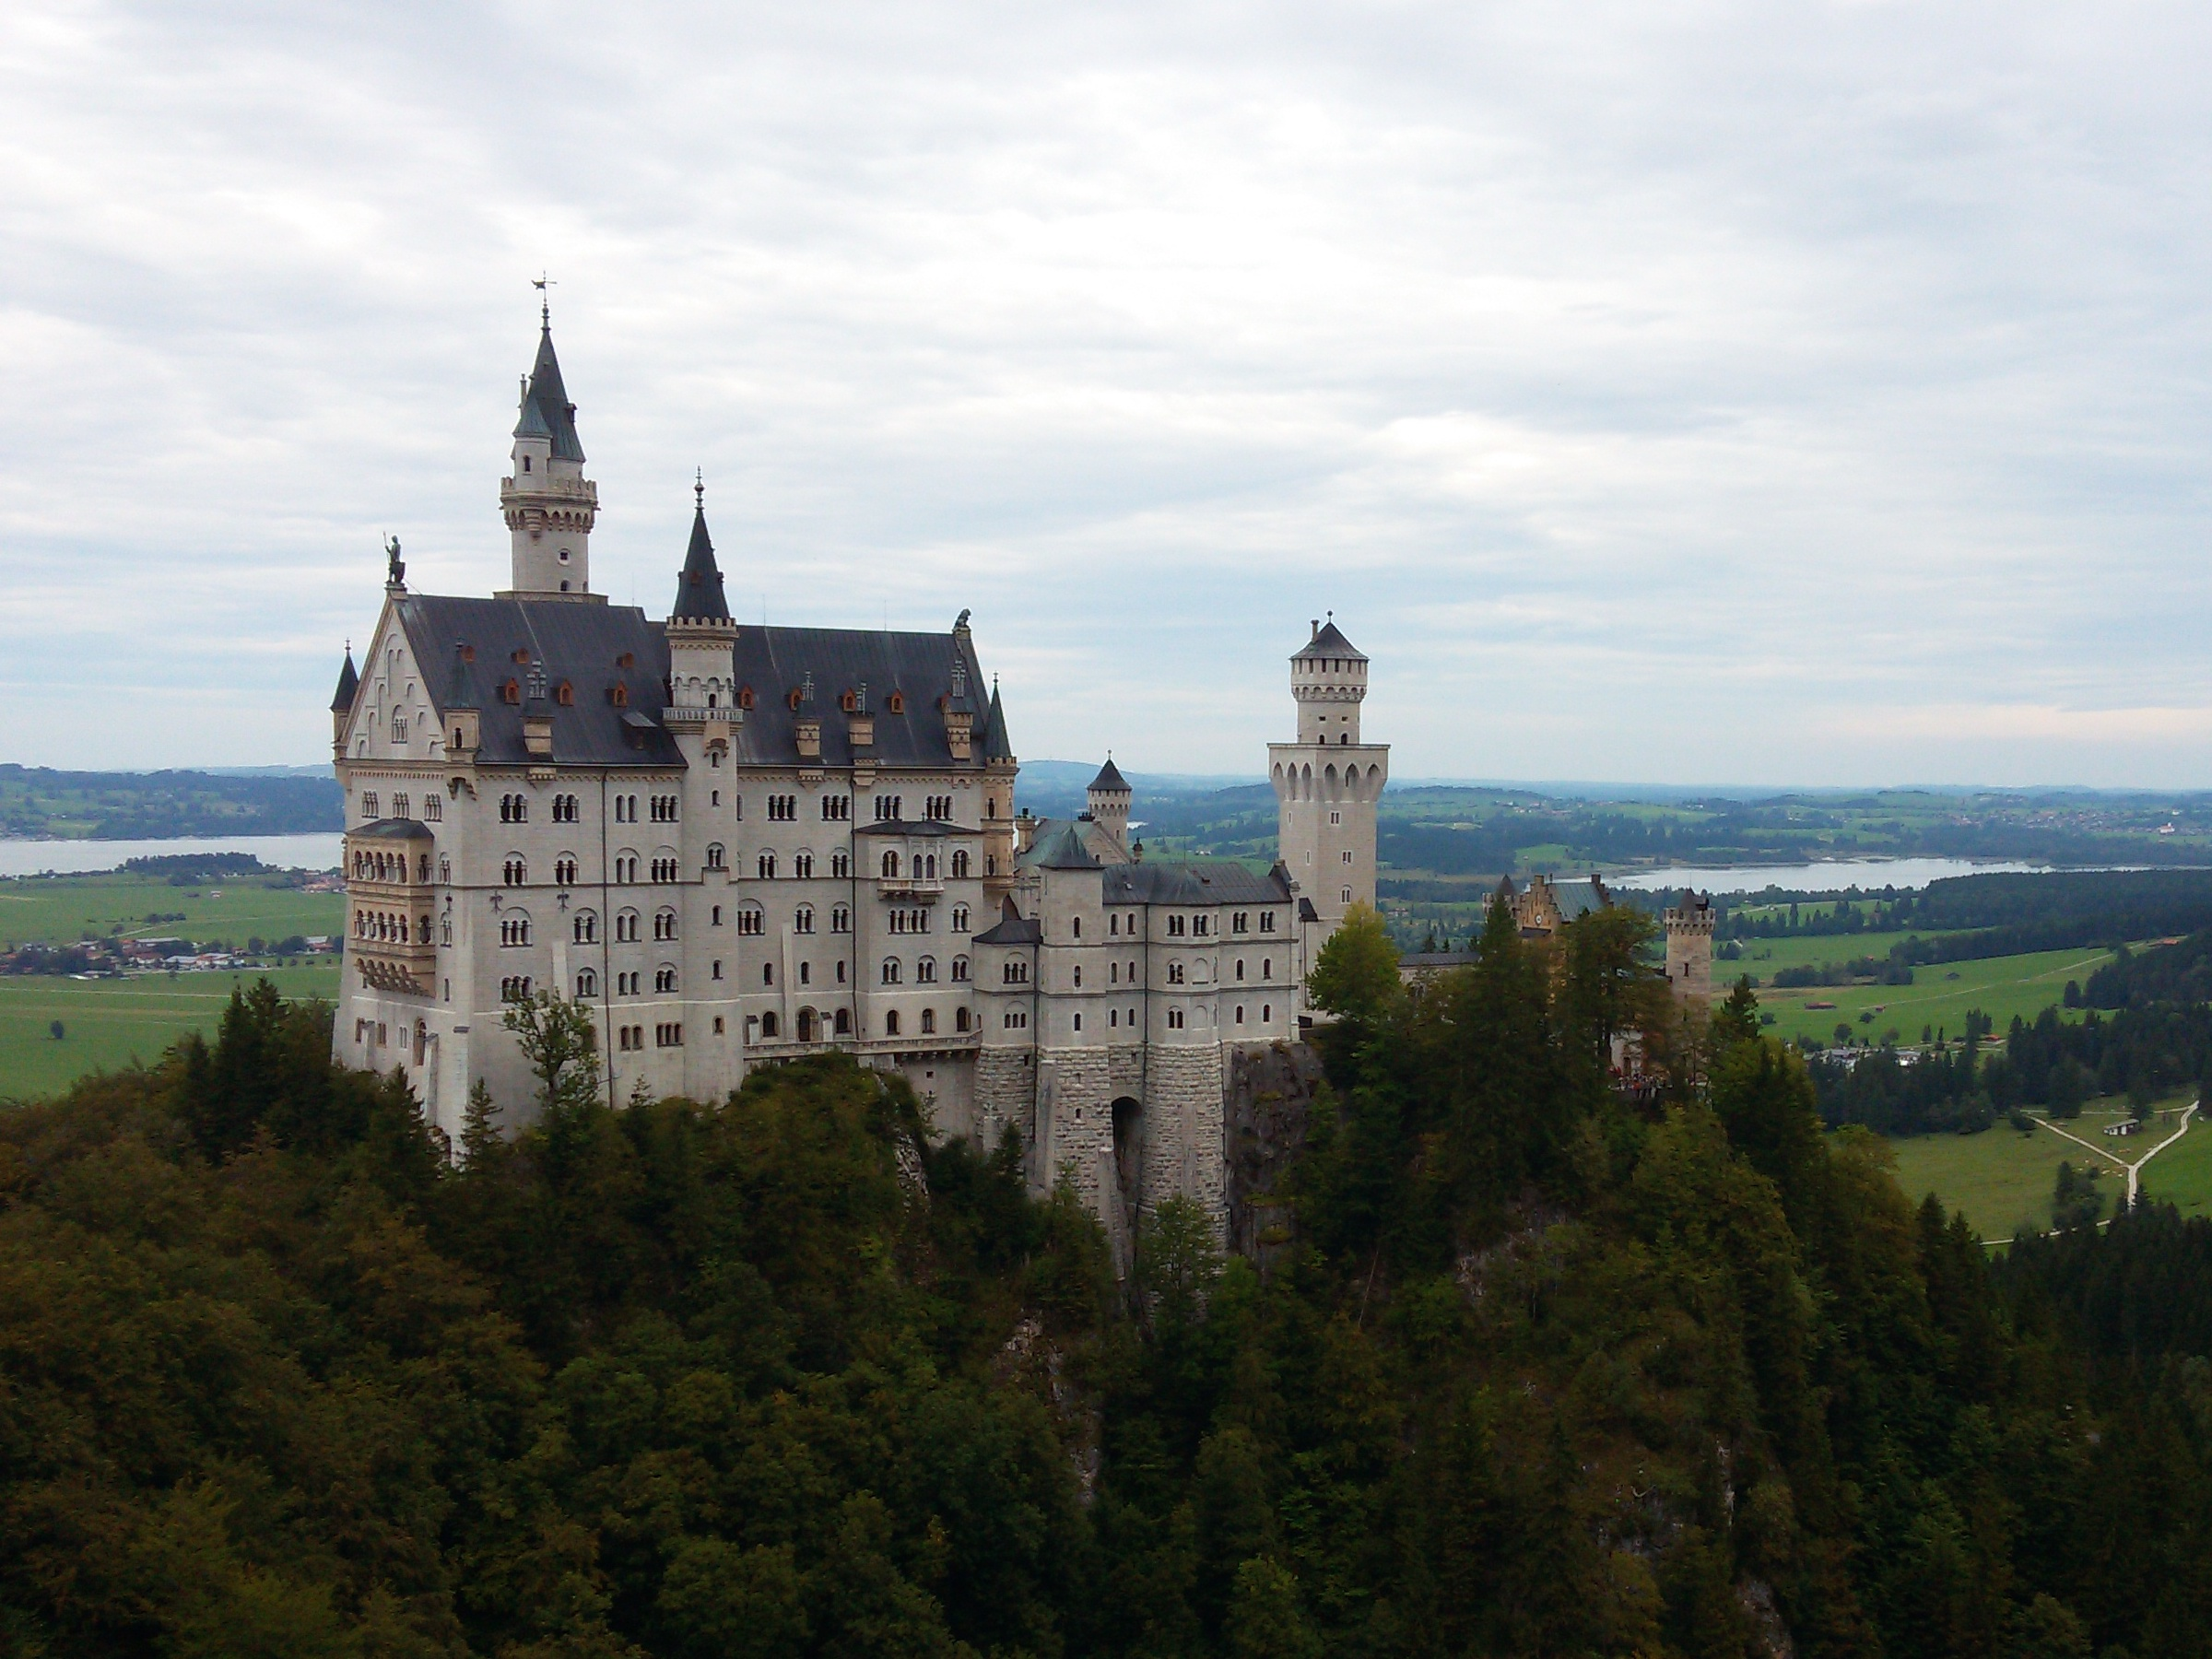
\includegraphics[width=0.8\textwidth]{castle0.jpg}
    \captionsetup{labelformat=empty}
    \caption{Малюнак 1: зыходная выява}
    \label{fig:sift0}
\end{figure}

\begin{figure}[t]
    \centering
    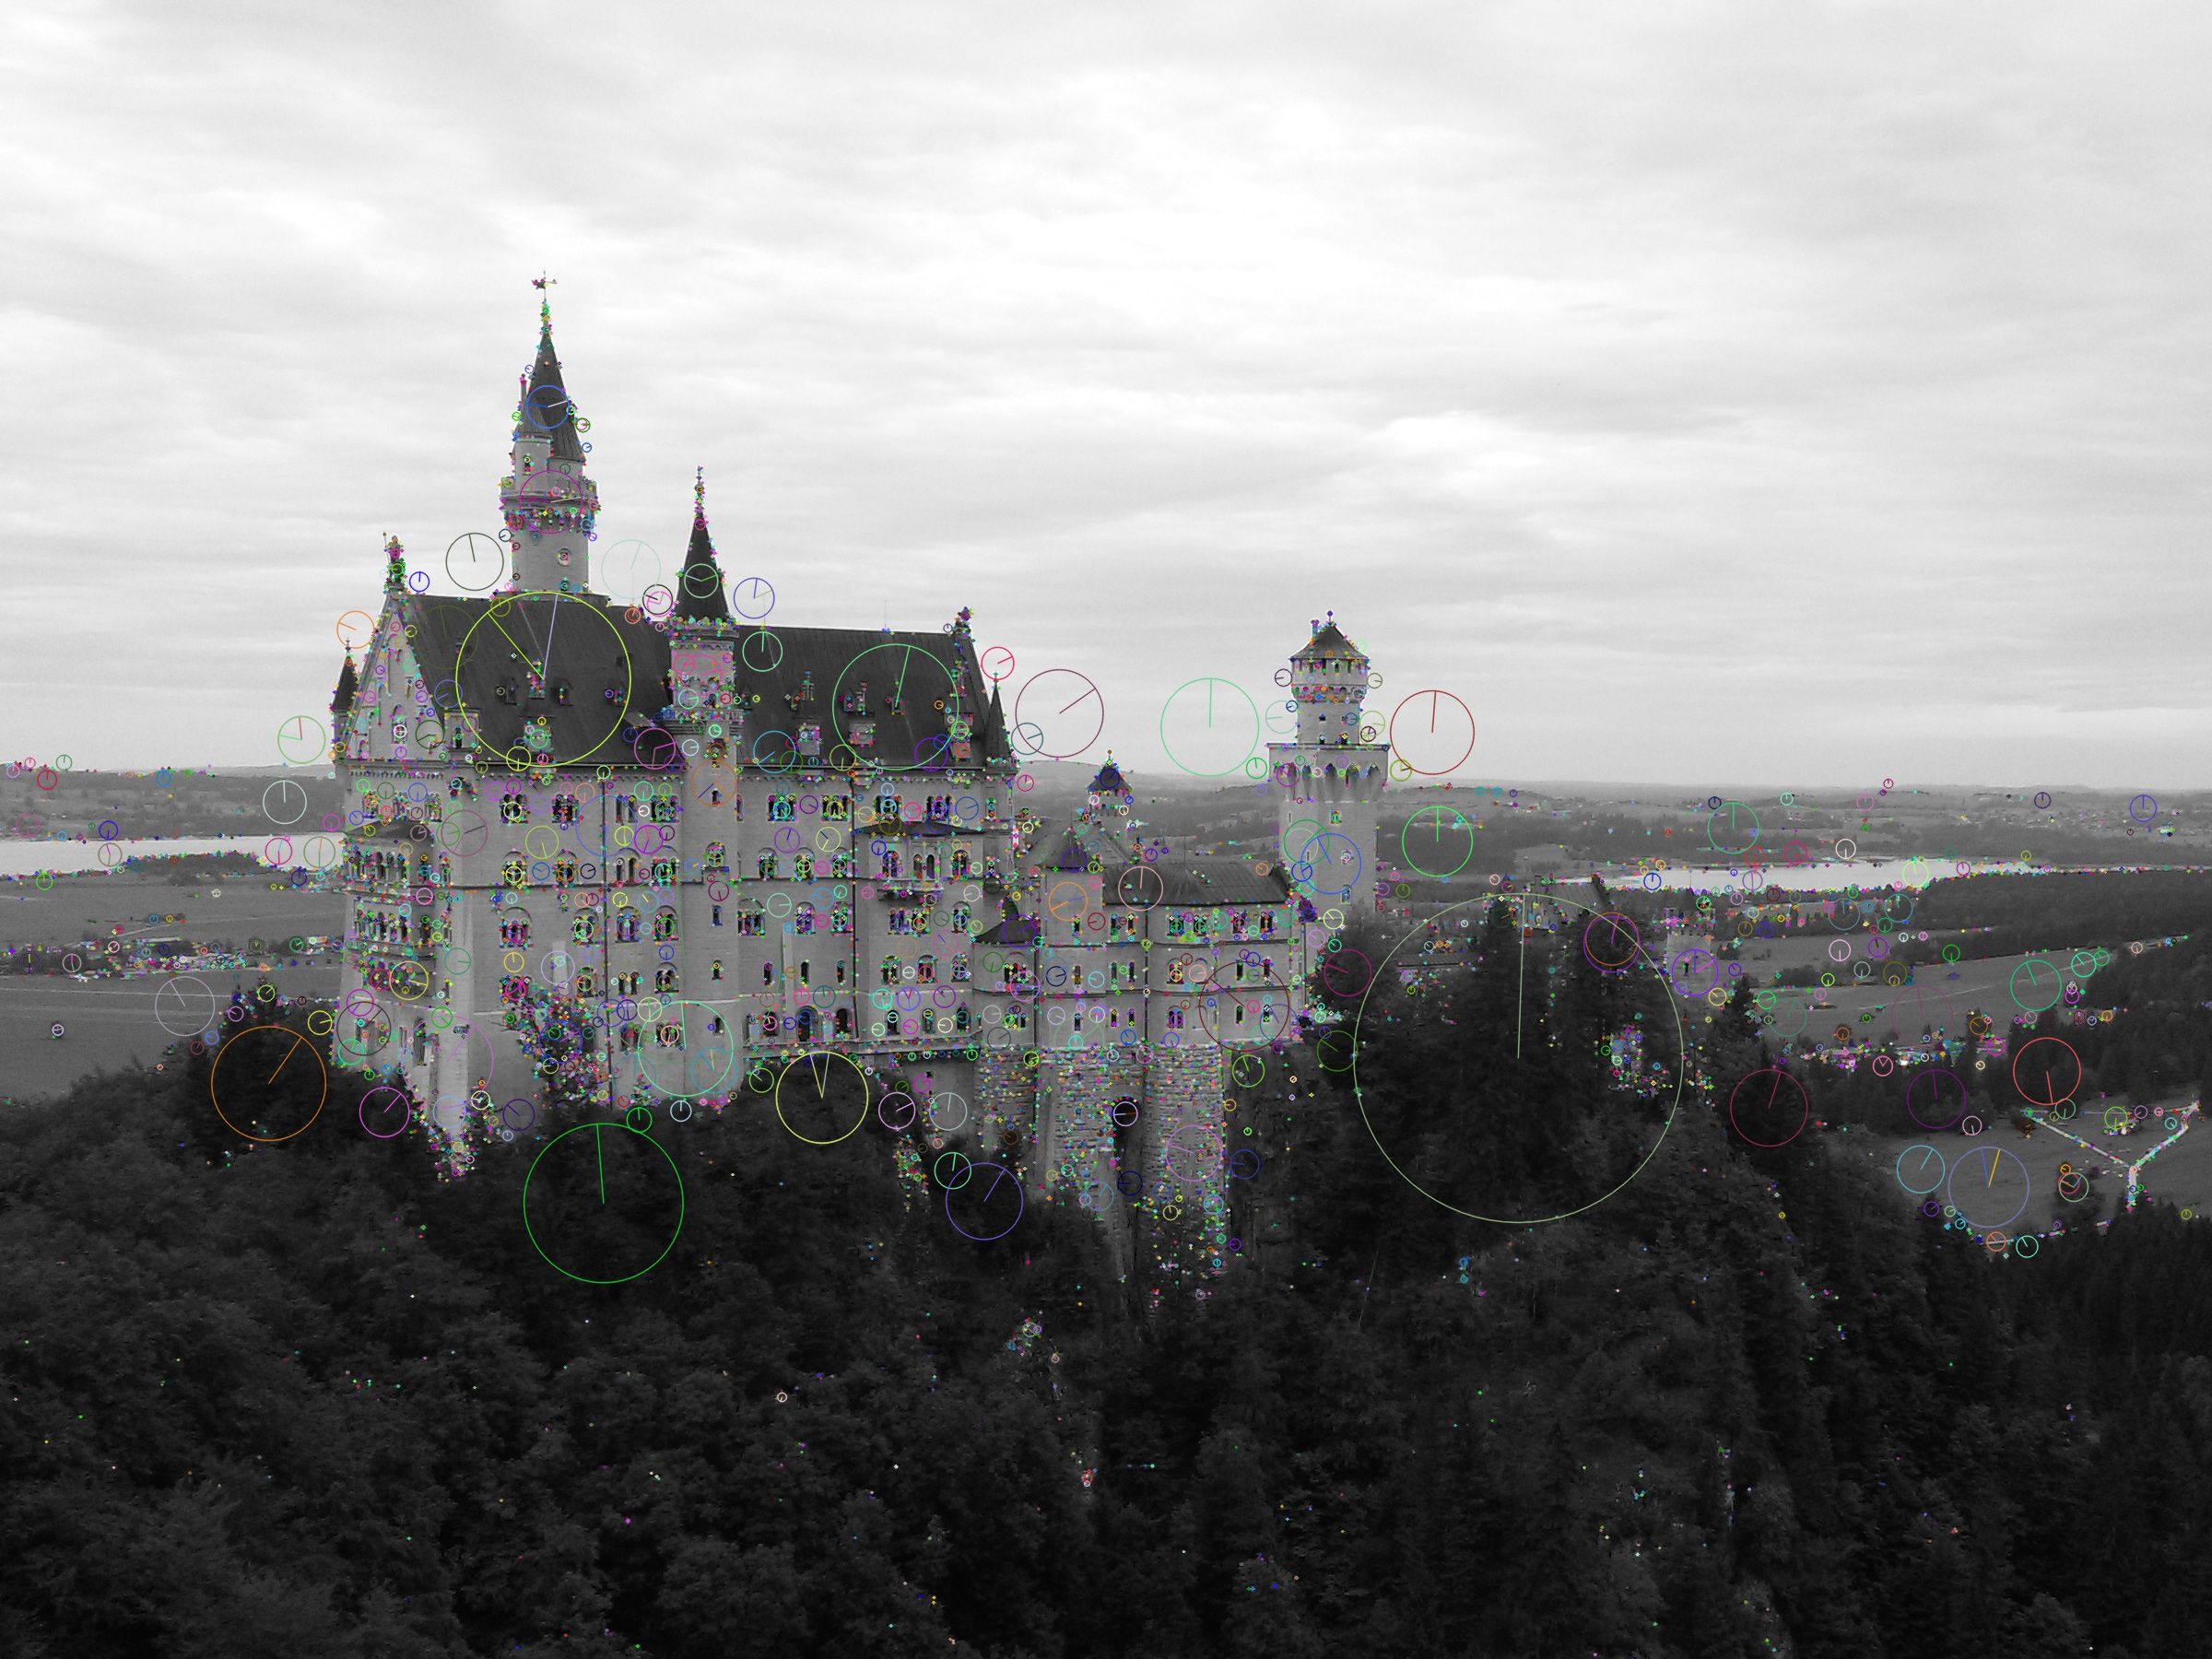
\includegraphics[width=0.8\textwidth]{castle0_sift.jpg}
    \captionsetup{labelformat=empty}
    \caption{Малюнак 2: выява з нанесенымі ключавымі кропкамі (SIFT)}
    \label{fig:sift1}
\end{figure}

Вылучэнне ключавых кропак на выяве з'яўляецца адной з базавых аперацыяў задачы апрацоўцы выяваў. Сутнасць у пошуку кропак, якія валодаюць вызначанымі ўласцівасцямі і ў пастаноўцы ім у адпаведнасць дэскрыптара, які апісывае гэтую кропку. Фармат дэскрыптара адрозніваецца ў залежнасці ад алгарытма, які мы прымяняем для вылучэння ключавых кропак.\par
Існуе вялікая колькасць алгарытмаў вылучэння ключавых кропак, якія могуць быць з рознай паспяховасцю прымененыя да адрозных набораў дадзеных. Напрыклад, для выяваў з вялікімі перападамі яскравасці і кантрасту можа быць эфектыўна прыменены алгарытм вылучэння межаў (англ. Edge detection) альбо алгарытм пошуку кутоў (англ. Corner detection). Найбольш распаўсюджанымі алгарытмамі агульнага прымянення з'яўляюцца SIFT, SURF, ORB і іншыя.\par 
На малюнку 2 можна бачыць візуалізацыю знойдзеных алгарытмам SIFT ключавых кропак.\par

\addcontentsline{toc}{subsection}{Спалучэнне ключавых кропак}
\subsection*{Спалучэнне адпаведных ключавых кропак}

\begin{figure}[h]
    \centering
    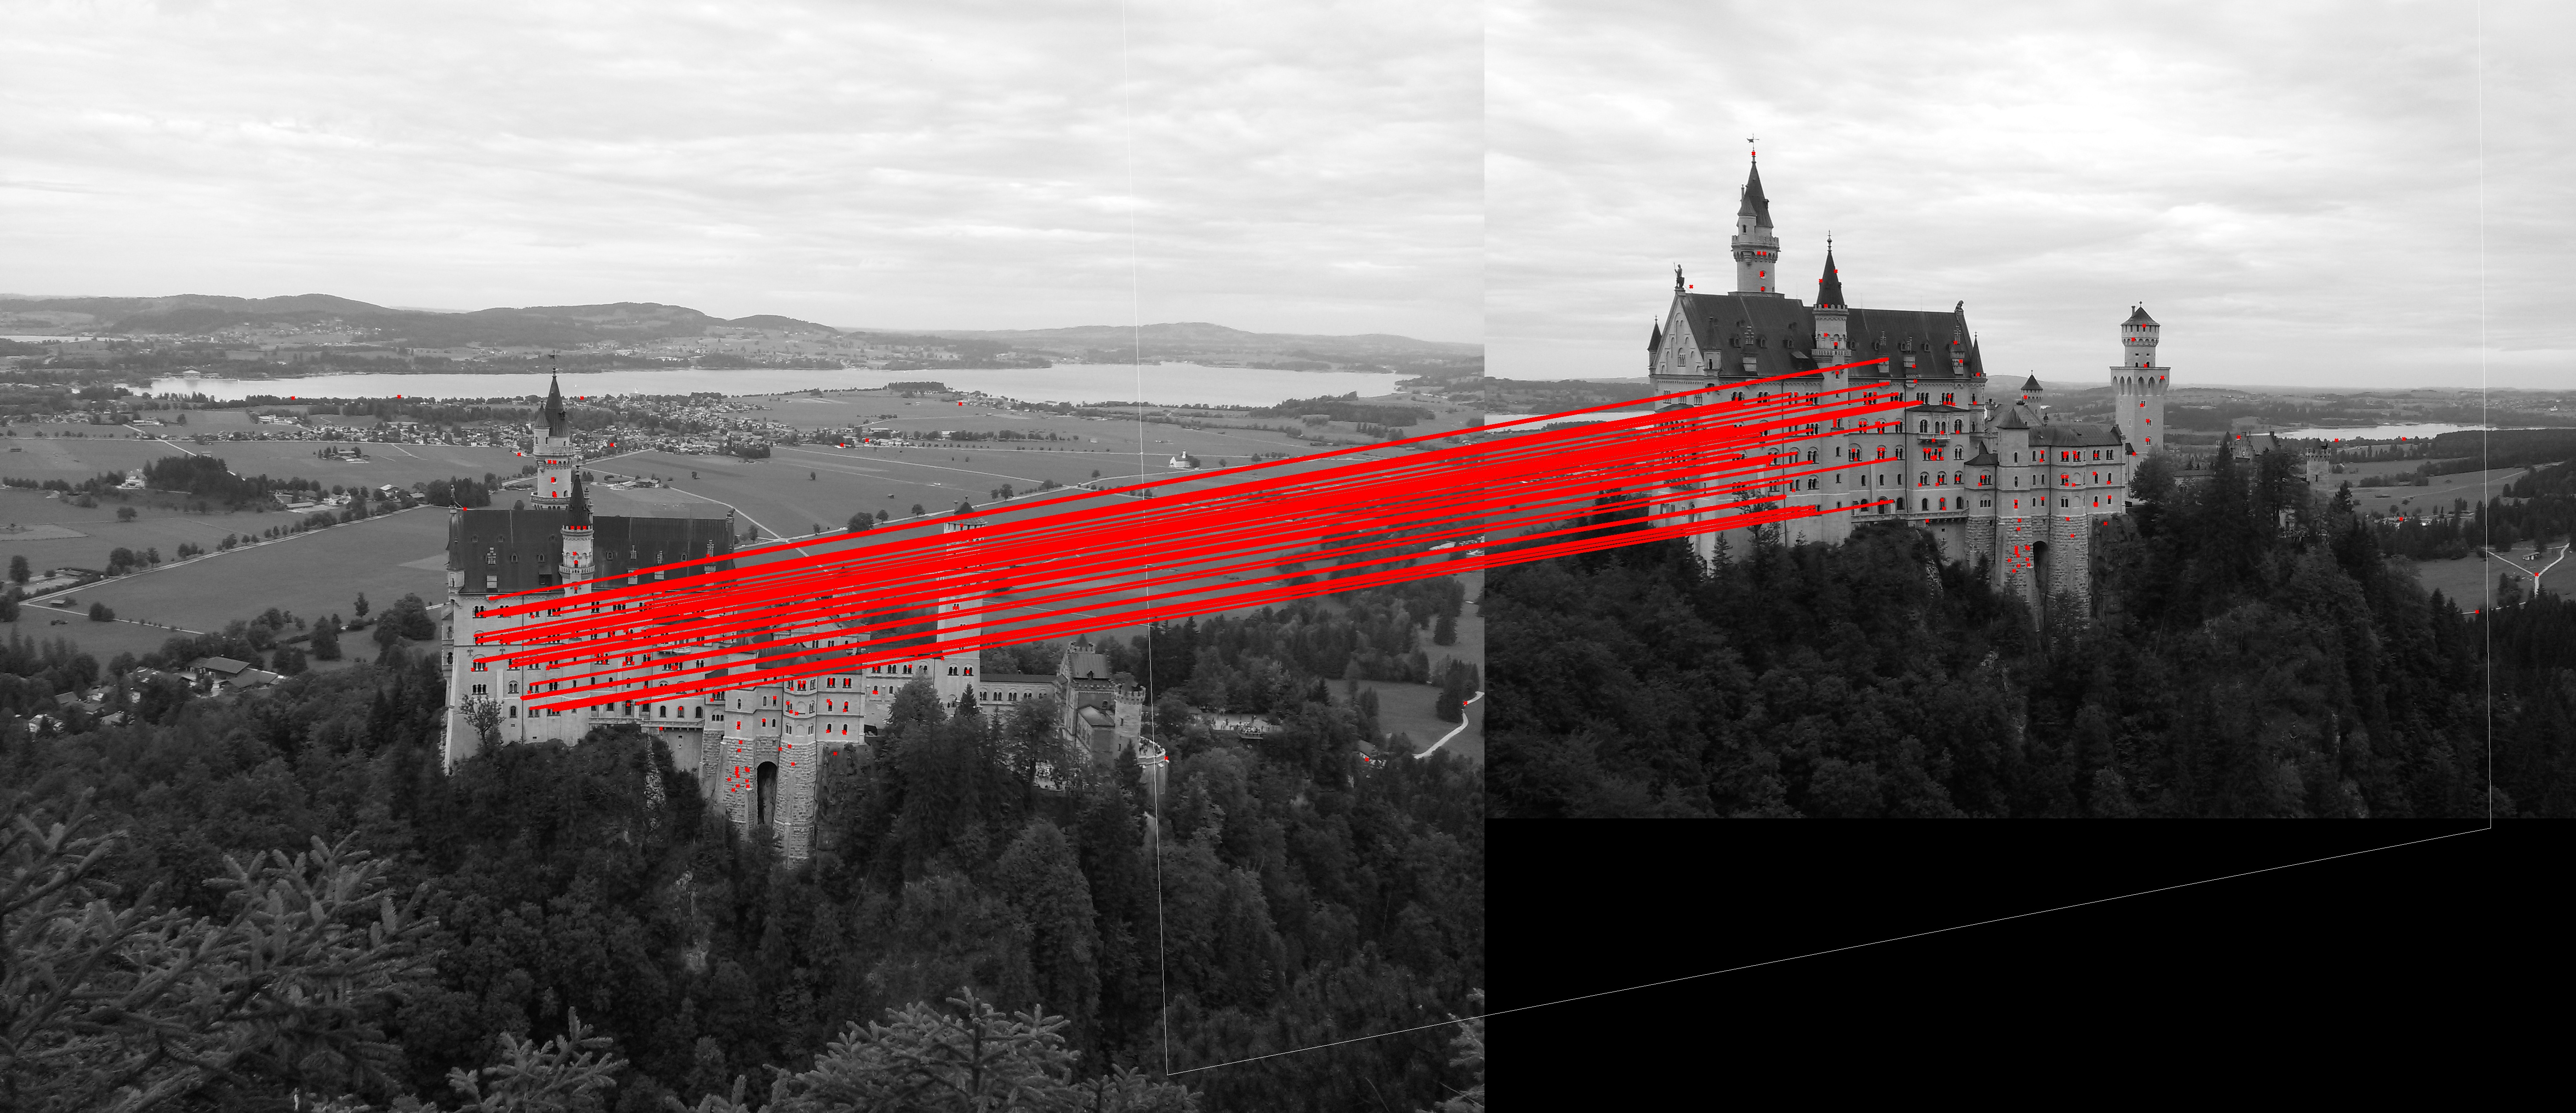
\includegraphics[width=1.0\textwidth]{castle_matches.jpg}
    \captionsetup{labelformat=empty}
    \caption{Малюнак 3: вынік пошуку адпаведнасцяў паміж ключавымі кропкамі}
    \label{fig:matches}
\end{figure}

Пасля таго, як для кожнай выявы з набора мы атрымалі мноства ключавых кропак, перад намі ставіцца задача пошуку кропак, якія адпавядаюць адным і тым жа кропкам у рэальнай прасторы. Праз тое, што кожная кропка апісываецца сваім дэскрыптарам, мы шукаем кропкі з найменшай адлегласцю паміж сабой (функцыя адлегласці вызначаецца у залежнасці ад таго, які тып дэскрыптара мы выкарыстоўваем) і аб'яўляем, што гэтыя пары (тройкі, і г.д.) кропак на выявах адпавядаюць адной кропцы ў прасторы. Такія мноствы кропак называюцца трэкамі.\par
Напрасцейшым шляхам пошуку адпаведнасцяў ёсць падлік адлегласці паміж усімі парамі кропак, упарадкаванне па росце адлегласці і выбар вызначанай колькасці найлепшых супадзенняў (англ. Brute Force Matching).\par
На малюнку 3 можна бачыць нанесеныя простыя лініі, якія злучаюць кропкі, адпаведныя адной і той жа кропцы прасторы. Дэскрыптары былі падлічаныя алгарытмам SIFT.
 
\addcontentsline{toc}{subsection}{Агульная задача рэканструкцыі паверхні}
\subsection*{Агульная задача рэканструкцыя паверхні}

\addcontentsline{toc}{subsubsection}{Асноўныя азначэнні і паняцці}
\subsubsection*{Асноўныя азначэнні і паняцці}
Пад рэканструкцыяй паверхні мы маем на ўвазе пабудову воблака кропак - мноства кропак у прасторы, якія суадносяцца паміж сабой як рэальныя, у выніку чаго воблака кропак дае нам уяўленне пра ўзаемнае размяшчэнне аб'ектаў на сцэне. Наступным этапам рэканструкцыі паверхні можа стаць "ушчыльненне" воблака і атрыманне сапраўднай трохмернай мадэлі, што, аднак, выходзіць за межы нашага праэкта. Спынімся падрабязней на пабудове разрэджанага воблака кропак. \par
У залежнасці ад набора дадзеных, якімі мы распараджаемся, задача рэканструкцыі можа адрознівацца. Пачнем з самай агульнай задачы. \par

\vspace{5mm}

{\bf Камера} - прылада, якая ажыццяўляе праэкцыю трохмернай кропкі на плоскасць. Пры наяўнасці ўсіх патрэбных для таго параметраў, мы можам паўтарыць праэкцыю. Кожная камера задаецца наступнымі параметрамі:
\begin{itemize}
    \item $f$ - фокусная адлегласць.
    \item $k1$, $k2$ - параметры скажэння.
    \item $R$ - $3 \times 3$ матрыца павароту.
    \item $t$ - $3 \times 1$ вектар зрушэння камеры адносна нейкай вызначанай кропкі прасторы.
\end{itemize} \par
Першыя два пункты адносяць да ўнутраных параметраў камеры, апошнія два - да вонкавых. Унутраныя параметры камеры вызначаюцца вытворцамі і не мяняюцца падчас выкарыстання камеры (хіба што ў выніку пэўнага фізічнага ўздзеяння). Вонкавыя ж параметры камеры вызначаюцца пазіцыяй камеры ў прасторы і ўнікальныя для кожнага ўнікальнага становішча камеры. \par
Такім чынам, для кожнай камеры справядлівыя наступныя ўраўненні:\\
Пераўтварэнне з міравых каардынатаў, у каардынаты камеры:
\begin{equation} \label{eq:world-to-camera}
    Q = RP + t,
\end{equation}
$P\in\mathbb{R}^3$ - кропка ў трохмернай прасторы.
\begin{equation} \label{eq:perspective-division}
    q = - \left( \begin{array}{ccc}
        Q_x / Q_z \\
        Q_y / Q_z \end{array} \right)
\end{equation}
Канверсія ў піксельныя каарданаты:
\begin{equation} \label{eq:to-pixel}
    p = f \cdot (1 + k_1 \cdot ||q||^2 + k_2 \cdot ||q||^4) \cdot q
\end{equation}

\addcontentsline{toc}{subsubsection}{Заданне матрыцы павароту праз кватэрніоны}
\subsubsection*{Заданне матрыцы павароту праз кватэрніоны}
Альтэрнатывай апісанай вышэй матрыцы павароту памера $3 \times 3$ можа быць апісанне павароту з дапамогай кватэрніонаў.\par
{\bf Кватэрніоны} - сістэма гіперкамплексных лікаў, якія ўтвараюць вектарную прастору размернасцю 4 над полем рэчаісных лікаў.\par
Кватэрніон можа быць прадстаўлены як фармальная сума $q(a, b, c, d) = a + bi + cj + dk$, дзе $a, b, c, d \in\mathbb{R}$, $i, j, k$ - уяўныя адзінкі, такія, што $i^2 = j^2 = k^2 = ijk = -1$.\par 
Кватэрніон часта запісываецца як пара $(a, \vec{u})$, дзе $a \in\mathbb{R}$, $\vec{u} = (b, c, d) \in\mathbb{R}^3$ - вектар у трохмернай прасторы, што дае нагоду задумацца аб прымяненні кватэрніонаў для заданняў паваротаў у трохмернай прасторы. \par
Негледзячы на тое, што кватэрніоны не знайшлі шырокага прымянення, іх выкарыстанне часта апраўданае ў некаторых галінах матэматыкі ды інфарматыкі, такіх як камп'ютарная графіка, навігацыя альбо праграмаванне гульняў. Кватэрніоны мінімальнай колькасцю скалярных параметраў задаюць паварот, пры гэтым яны пазбаўленыя выраджанасці, якая сустракаецца пра заданні паварота пры дапамозе толькі трох параметраў (напрыклад - вугламі Эйлера). \par
Няхай маем кватэрніон $q = (w, x, y, z)$, тады матрыца павароту можа быць запісаная праз кватэрніон як:
\begin{equation} \label{eq:quaternion-to-rotation}
    R = \left( \begin{array}{ccc}
    1 - 2y^2 - 2z^2 & 2xy - 2zw & 2xz + 2yw \\
    2xy + 2zw & 1 - 2x^2 - 2z^2 & 2yz - 2xw \\
    2xz - 2yw & 2yz + 2xw & 1 - 2x^2 - 2y^2 \end{array} \right)
\end{equation}

Праз гэтую формулу пераходзім ад павароту камеры, запісанага з дапамогай квартэніона, да формулаў \eqref{eq:world-to-camera} - \eqref{eq:to-pixel}.

\addcontentsline{toc}{subsubsection}{Пастаноўка задачы рэканструкцыі}
\subsubsection*{Пастаноўка задачы рэканструкцыі}
Задача аднаўлення трохмерных каардынатаў кропак па наборы выявах, зробленых з розных ракурсаў і пазіцый, атрымала агульную назву задачы пучковай аптымізацыі (англ. {\bf bundle adjustment}). Задача заключаецца ў мінімізацыі памылкі функцыянала, які задае суадносіны паміж мноствам кропак прасторы і праэкцыямі гэтых кропак. Строга гэта можа быць запісана як:
\begin{equation} \label{eq:bundle-adjustment}
    \min_{a_j, b_i} \sum_{i=1}^{n} \sum_{j=1}^{m} v_{ij}d(Q(a_j, b_i), x_{ij})^2
\end{equation}
дзе:\\
$n$ - колькасць кропак у трохмернай прасторы, якія бачныя хаця б на адным фотаздымку,\\
$m$ - колькасць выяваў (колькасць камер),\\
$x_{ij}$ - праэкцыя кропкі $i$ на выяву $j$,\\
$v_{ij}$ - дваічная зменная, якая вызначае, ці бачная кропка $i$ на выяве $j$,\\
$a_{j}$ - вектар параметраў камеры $j$,\\
$b_{i}$ - набліжэнне для кропкі $i$ прасторы,\\
$Q(a_j, b_i)$ - функцыя пошуку праэкцыі кропкі $i$ на выяву $j$,\\
$d(x, y)$ - Эўклідава адлегласць паміж кропкамі $x$ i $y$.\par
Мінімізаваўшы памылку функцыянала, мы знойдзем найлепшае магчымае набліжэнне для параметраў камераў $a_{j}$ і кропак трохмернай прасторы $b_{i}$, што дасць нам магчымасць зрабіць візуалізацыю мадэлі, што і з'яўляецца нашай мэтай.\par
Вышэй, у формулах \eqref{eq:world-to-camera} - \eqref{eq:to-pixel} мы ўжо разгледзелі, што ўяўляе сабой функцыя пошуку праэкцыі $Q(a_j, b_i)$.\par
Дадзеная задача можа рашацца як агульнымі падыходамі да мінімізацыі функцыяналу, так і спецыяльна распрацаванымі алгарытмамі, якія ўлічваюць разрэджаную структуру матрыцы, якая апісвае функцыянал, такім чынам эфектыўна рашаючы задачу пучковай аптымізацыі. Алгарытмам, які атрымаў найбольшы распаўсюд пры практычнай рэалізацыі, з'яўляецца алгарытм Левенберга-Марквардта (англ. Levenberg–Marquardt algorithm, LMA). Гэта ітэратыўны алгарытм рашэння задачы мінімізацыі нелінейнага функцыянала спосабам найменшых квадратаў (англ.  non-linear least squares problem).

\addcontentsline{toc}{subsection}{Асаблівасці задачы рэканструкцыі па дадзеных з БПЛА}
\subsection*{Асаблівасці задачы рэканструкцыі па дадзеных з беспілотных лятальных апаратаў}
Той факт, што рэканструкцыя адбываецца не на выпадковым наборы дадзеных, пра які няма ніякай дадатковай інфармацыі, дае нам прастору для аптымізацыі працэса рэканструкцыі: скарачэння часу і паляпшэння якасці пабудаванай мадэлі. Пералічым асаблівасці нашай задачы ў пераўнанні з агульнай задачай:
\begin{itemize}
    \item Усе здымкі зробленыя адной фізічнай камерай, такім чынам унутраныя параметры ўсіх камераў застаюцца нязменнымі. Больш за тое, унутраныя камеры параметры застаюцца нязменнымі не толькі ў межах аднаго набора, але і для ўсіх здымкаў зробленым адным БПЛА з фіксаванай на ім камерай. Гэты факт не ўносіць зменаў у працэс рэканструкцыі, але спрашчае працэс карыстання БЛПА на практыцы (адсутнасць патрэбы ў шторазовым калібраванні для высвятлення ўнутраных параметраў камеры).
    \item Апроч камеры ў нашым распараджэнні, у залежнасці ад канфігурацыі БПЛА, могуць мецца і іншыя датчыкі: акселерометр, гіраскоп, GPS-датчык і інш. Дадзеныя сабраныя імі, могуць выкарыстоўвацца як для вызначэння вонкавых параметраў камеры, так і для папярэдняга размяшчэння кропак у прасторы.
\end{itemize}

\subsubsection*{Змены ў набор дадзеных і алгарытмы з улікам вышэйсказанага}
Прычыны, па якіх дадатковыя дадзеныя станоўча паўплываюць на якасць і хуткасць рэканструкцыі, абсалютна натуральныя: памяншэнне колькасці параметраў і больш якасная пачатковая апраксімацыя. Такім чынам мы маем два падыходы да выкарыстання дадзеных, якімі суправаджаецца набор выяваў:
\begin{itemize}
    \item Аб'яўленне параметраў канстантнымі і непасрэдная іх падстаноўка ва ўраўненні - такім чынам, маем яўнае памяншэнне колькасці параметраў што не можа не паўплываць на хуткасць адпрацоўкі алгарытма і на выніковае значэнне памылкі праэкцыі станоўча. Відавочны і недахоп: немагчымасць дакладнага задання параметраў і наступнае аб'яўленне іх канстантнымі прывядзе да псавання канчатковых значэнняў трохмерных кропак і, адпаведна, пагаршэння якасці пабудаванай мадэлі. Дакладнасць вызначэння параметраў знаходзіцца ў простай залежнасці ад карэктнасці пабудаванай мадэлі. На практыцы высвятляецца, што такі падыход вядзе да значнага пагаршэння канчатковых вынікаў і кепска прымяняльны на рэальных дадзеных.
    \item Выкарыстанне дадатковых дадзеных для пачатковай апраксімацыі значэнняў параметраў камеры і палажэнняў кропак у прасторы. Пры такім падыходзе, мы не рызыкуем стаць ахвярамі кепскай дакладнасці альбо памылак у апісанні дадзеных - разам з тым, колькасць ітэрацый у працэсе пучковай аптымізацыі можа паменшыцца ў разы. Гэты падыход можа паспяхова быць прыменены на практыцы: хуткасць працэса пабудовы проста залежыць ад якасці ўваходных дадзеных - яўных жа памылак у выніковай мадэлі (такіх, як у першым пункце) назірацца не будзе, праз тое, што алгарытм выправіць яўна хібныя ўваходныя дадзеныя.
\end{itemize}
Альтэрнатывай можа стаць змяшаны падыход: напрыклад, аб'явіць фокусную адлегласць пастаяннай і недаступнай да зменаў (калі мы дастаткова ўпэўненыя ў лічбах, якія прадастаўляе вытворца камера, альбо атрыманых у выніку каліброўцы), але дазволіць алгарытму удакладняць параметры павароту камеры - пры дастаткова дакладных пачатковых значэннях яны будуць змененыя нязначна. 

\newpage